% http://tug.ctan.org/tex-archive/macros/latex/contrib/drawstack/
% http://www.ctan.org/pkg/bytefield


\documentclass{article}

\usepackage{drawstack}

\usepackage{bytefield}

% Use this instead if you don't want colors.
% \usepackage[nocolor]{drawstack}

\title{{\tt drawstack.sty}: Draw execution stack easily in LaTeX}
\author{Matthieu Moy}

\begin{document}
\maketitle

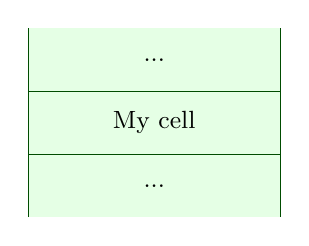
\begin{tikzpicture}[scale=0.8]
	\small
	\stacktop{}
	\cell{My cell}

	\stackbottom{}
\end{tikzpicture}



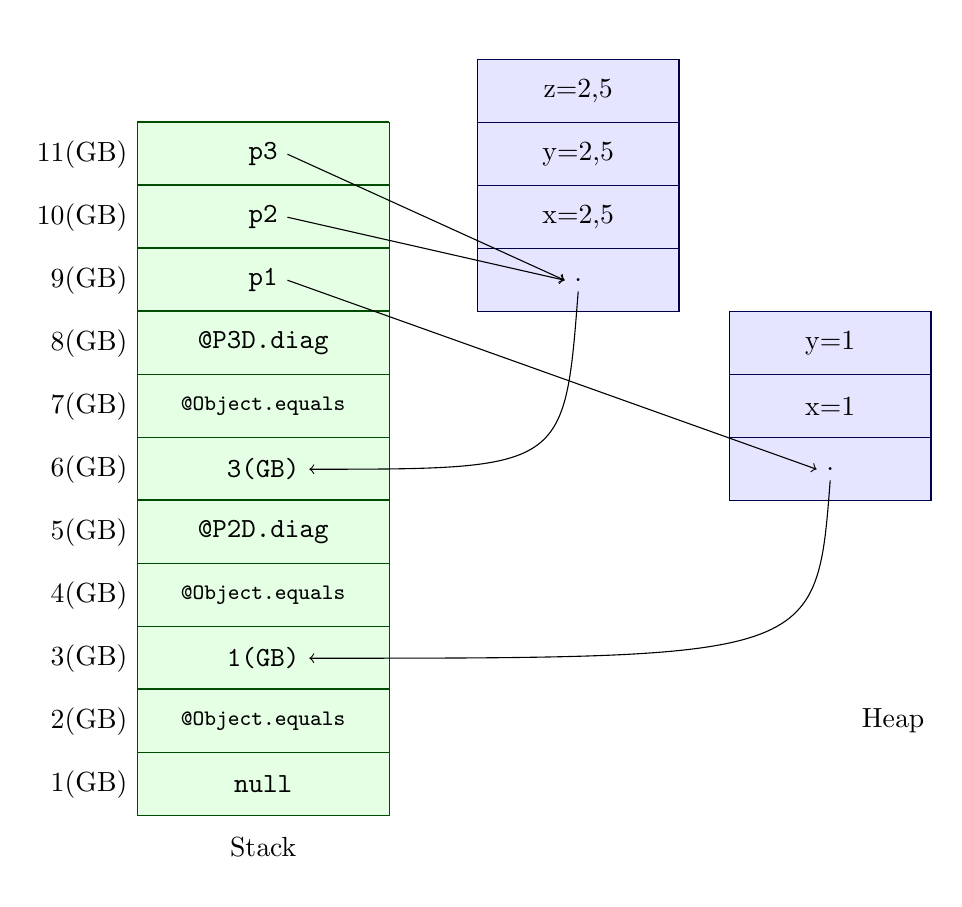
\begin{tikzpicture}[scale=0.8]
%\stacktop{}
	\separator
	\cell{\texttt{p3}}        \cellcomL{11(GB)} \coordinate (p3) at (currentcell.east);
	\separator
	\cell{\texttt{p2}}        \cellcomL{10(GB)} \coordinate (p2) at (currentcell.east);
	\separator
	\cell{\texttt{p1}}        \cellcomL{ 9(GB)} \coordinate (p1) at (currentcell.east);
	\separator
	\cell{\texttt{@P3D.diag}} \cellcomL{ 8(GB)}
	\cell{\texttt{\footnotesize @Object.equals}} \cellcomL{ 7(GB)}
	\cell{\texttt{3(GB)}}     \cellcomL{ 6(GB)} \coordinate (T1) at (currentcell.east);
	\separator
	\cell{\texttt{@P2D.diag}} \cellcomL{ 5(GB)}
	\cell{\texttt{\footnotesize @Object.equals}} \cellcomL{ 4(GB)}
	\cell{\texttt{1(GB)}}     \cellcomL{ 3(GB)} \coordinate (T2) at (currentcell.east);
	\separator
	\cell{\texttt{\footnotesize @Object.equals}} \cellcomL{ 2(GB)}
	\cell{\texttt{null}}      \cellcomL{ 1(GB)}
	\cell[draw=none]{Stack}


	\drawstruct{(5,1)})
	\structcell{z=2,5}
	\structcell{y=2,5}
	\structcell{x=2,5}
	\structcell{.} \coordinate (O1) at (currentcell.west);
	\coordinate (O1l) at (currentcell.south);

	\drawstruct{(9,-3)}
	\structcell{y=1}
	\structcell{x=1}
	\structcell{.} \coordinate (O2) at (currentcell.west);
	\coordinate (O2l) at (currentcell.south);

	\draw[->] (p3) -- (O1);
	\draw[->] (p2) -- (O1);
	\draw[->] (p1) -- (O2);

	\draw[->] (O1l) .. controls (O1 |- T1) .. (T1);
	\draw[->] (O2l) .. controls (O2 |- T2) .. (T2);

	\draw (10,-10) node{Heap};

\end{tikzpicture}


\newpage

\title{Integrating \texttt{bytefield} and \texttt{hyperref}}
\author{Scott Pakin}

\newpage

\begin{bytefield}{32}
\bitheader{0-31} \\
\bitbox{4}{Four} & \bitbox{8}{Eight} &
\bitbox{16}{Sixteen} & \bitbox{4}{Four}
\end{bytefield}

\newpage

\begin{bytefield}[endianness=big,bitwidth=2em]{16}
\bitheader[lsb=16]{16-31} \\
\bitbox{1}{\tiny Enable} & \bitbox{7}{Reserved}
& \bitbox{8}{Bus} \\[3ex]
\bitheader{0-15} \\
\bitbox{5}{Device} & \bitbox{3}{Function} & \bitbox{6}{Register}
& \bitbox{2}{00}
\end{bytefield}

\newpage

\definecolor{lightgray}{gray}{0.8}
\begin{bytefield}{32}
\bitheader{0,4,8,12,16,20,24,28} \\
\bitbox{8}{Tag} & \bitbox{8}{Value} &
\bitbox{4}{\color{lightgray}\rule{\width}{\height}} &
\bitbox{12}{Mask} \\
\wordbox{1}{Key}
\end{bytefield}

\newpage

% \newcommand{\bitlabel}[2]{%
% \bitbox[]{#1}{%
% \raisebox{0pt}[4ex][0pt]{%
% \turnbox{45}{\fontsize{7}{7}\selectfont#2}%
% }%
% }%
% }

% \begin{bytefield}[bitwidth=1em]{16}
%   \bitlabel{1}{Carry} & \bitlabel{1}{Reserved} &
%   \bitlabel{1}{Parity} & \bitlabel{1}{Reserved} &
%   \bitlabel{1}{Adjust} & \bitlabel{1}{Reserved} &
%   \bitlabel{1}{Zero} & \bitlabel{1}{Sign} &
%   \bitlabel{1}{Trap} & \bitlabel{1}{Interrupt enable} &
%   \bitlabel{1}{Direction} & \bitlabel{1}{Overflow} &
%   \bitlabel{2}{I/O privilege level (12--13)} &
%   \bitlabel{1}{Nested task} & \bitlabel{1}{Reserved} \\
%   \bitheader{0-15} \\
%   \bitbox{1}{0} & \bitbox{1}{1} & \bitbox{1}{0} & \bitbox{1}{0} &
%   \bitbox{1}{0} & \bitbox{1}{0} & \bitbox{1}{0} & \bitbox{1}{1} &
%   \bitbox{1}{0} & \bitbox{1}{1} & \bitbox{1}{0} & \bitbox{1}{0} &
%   \bitbox{1}{0} & \bitbox{1}{0} & \bitbox{1}{0} & \bitbox{1}{0}
% \end{bytefield}


\newpage

\newcommand{\colorbitbox}[3]{%
\rlap{\bitbox{#2}{\color{#1}\rule{\width}{\height}}}%
\bitbox{#2}{#3}}
\definecolor{lightcyan}{rgb}	{0.80, 	0.90   , 1   }
\definecolor{lightgreen}{rgb}	{0.50, 	1   , 0.50}
\definecolor{lightred}{rgb}		{1   , 	0.70, 0.71}
\definecolor{lightblue}{rgb}	{0   , 	0.90, 1   }

\begin{bytefield}[bitheight=\widthof{-CP-},
	boxformatting={\centering\small}]{32}
	\bitheader[endianness=big]{31,23,0} \\
	\colorbitbox{lightcyan}{1}{\rotatebox{90}{CP}} &
	\colorbitbox{lightcyan}{8}{display} &
	\colorbitbox{lightblue}{23}{datos estáticos}
	\colorbitbox{lightred}{23}{Mantissa}
\end{bytefield}

\newpage

\newcommand{\fakesixtyfourbits}[1]{%
\tiny
\ifnum#1=1234567890
#1
\else
\ifnum#1>9
\count32=#1
\advance\count32 by 48
\the\count32%
\else
\ifnum#1<4
#1%
\else
\ifnum#1=6
$\cdots$%
\fi
\fi
\fi
\fi
}
\begin{bytefield}[%
bitwidth=\widthof{\tiny Fwd~},
bitformatting=\fakesixtyfourbits,
endianness=big]{16}
\bitheader{0-15} \\
\bitbox{1}{\tiny F/E} & \bitbox{1}{\tiny T0} & \bitbox{1}{\tiny T1}
& \bitbox{1}{\tiny Fwd} & \bitbox{12}{Data value}
\end{bytefield}


\newpage




\begin{bytefield}[endianness=little,bitwidth=0.11111\linewidth]{9}
	\bitheader[endianness=little,]{0-9} \\
	\colorbitbox{white}{1}{8} &
	\colorbitbox{lightgreen}{1}{4} &
	\colorbitbox{lightgreen}{1}{?} &
	\colorbitbox{lightgreen}{1}{?} &
	\colorbitbox{lightcyan}{2}{par1} &
	\colorbitbox{lightcyan}{2}{par2} &
	\colorbitbox{lightcyan}{1}{res} &
	\colorbitbox{lightred}{1}{527}
\end{bytefield}


\newpage

% \begin{bytefield}[endianness=little,bitwidth=0.10\linewidth]{9}
% 	\bitheader[endianness=little,]{0-9} \\
% 	\colorbitbox{white}{1}{8} &
% 	\colorbitbox{lightgreen}{1}{4} &
% 	\colorbitbox{lightgreen}{1}{?} &
% 	\colorbitbox{lightgreen}{1}{?} &
% 	\colorbitbox{lightcyan}{2}{par1} &
% 	\colorbitbox{lightcyan}{2}{par2} &
% 	\colorbitbox{lightcyan}{1}{res} &
% 	\colorbitbox{lightred}{1}{527}
% \end{bytefield}


\end{document}
